\documentclass[11pt,a4paper]{article}
\usepackage[T1]{fontenc}
\usepackage[margin=2.3cm]{geometry}
\usepackage{amsmath,amssymb}
\usepackage{graphicx}
\usepackage[dvipsnames]{xcolor}
\usepackage{enumitem}
\usepackage[colorlinks=true,linkcolor=blue,urlcolor=blue]{hyperref}
\setlength{\parskip}{0.6em}
\setlength{\parindent}{0pt}
\begin{document}

\begin{center}{\LARGE\bfseries openmole}\\[0.4em]{\large Balance a reaction and work out how much reagent you need, in three sessions.}\\[0.2em]\small PAN IIT OSS explainer \textbullet{} secondary school to diploma / undergraduate (levels 3-5)\end{center}

\section*{Why this exists}
Every chemical process, from a fertiliser plant to a cooking flame, is bookkeeping with atoms. This explainer shows the mathematics behind balancing equations and counting reagents, using only counting, ratios and one matrix idea, so you can build it yourself.

\section*{The end goal}
Balance a reaction and compute how much reagent you need (stoichiometry). The end goal is stoichiometry as used by chemists and process engineers: balance a reaction, convert between grams and moles, find the limiting reagent and compute how much reagent you need. The same mass-balance logic is used for furnaces, reactors, water treatment and fuel calculations.

\section*{How the three sessions build up}
\begin{enumerate}[nosep]
\item \textbf{Session 1: Atoms are conserved: balancing is bookkeeping} (Level 1, conceptual interactive model, 60 min).
\item \textbf{Session 2: From a balanced equation to grams} (Level 2, mathematical engineering model, 75 min).
\item \textbf{Session 3: An automatic balancer and a reactor sweep} (Level 3, simulation and validation, 90 min).
\end{enumerate}

\section{Session 1: Atoms are conserved: balancing is bookkeeping}

\subsection*{A. Real-world problem}
A recipe says 2 slices of bread and 1 slice of cheese make 1 sandwich. Double the sandwiches and you double every ingredient, but you never create or lose a slice. A chemical reaction is a recipe whose ingredients are atoms: when hydrogen burns in oxygen to make water, no atom appears or disappears, they only regroup. So how many hydrogen molecules and oxygen molecules do you need, and how many water molecules do you get? This session is general education about the arithmetic; do not try these reactions yourself at home.

\subsection*{B. Concept and theory}
A formula tells how many atoms of each element a molecule has: in H2O the small number after a symbol is the count (H2 means 2 atoms, no number means 1), and brackets multiply what is inside, so Ca(OH)2 has 1 Ca, 2 O and 2 H. In an equation, a big number in front of a formula (the coefficient) says how many molecules of that substance take part, and it multiplies every atom in the formula. Because atoms are only regrouped, the total number of atoms of each element must be the same on the left and on the right. Never change the small numbers inside a formula to balance: that changes the substance (H2O2 is not water). Only the coefficients may be changed. Multiplying every coefficient by the same number gives the same recipe made several times over.

\begin{itemize}[nosep]
\item a, b, c: coefficients (how many H2, O2 and H2O molecules) (no unit (a count))
\item N\_X: total number of atoms of element X on one side (atoms (a count))
\item x\_i,X: atoms of X in one molecule of species i (the small number) (atoms per molecule)
\item c\_i: coefficient of species i (molecules (a count))
\end{itemize}

\begin{equation*}
2\,\mathrm{H_2}+\mathrm{O_2}\;\longrightarrow\;2\,\mathrm{H_2O}
\end{equation*}

\begin{equation*}
N_X^{\text{left}}=\sum_{i\in\text{reactants}}c_i\,x_{i,X}\qquad N_X^{\text{right}}=\sum_{i\in\text{products}}c_i\,x_{i,X}
\end{equation*}

\begin{equation*}
\text{balanced}\iff N_X^{\text{left}}=N_X^{\text{right}}\ \text{for every element }X
\end{equation*}

\begin{center}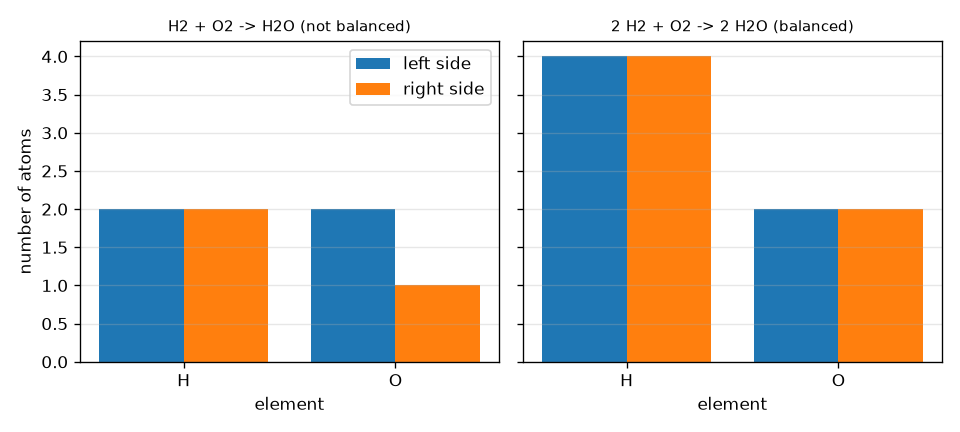
\includegraphics[width=0.85\linewidth]{figures/s01_atom_counts.png}\\\small Atom counts on the left and right: the unbalanced and the balanced recipe for water.\end{center}

\subsection*{E. Worked example}
Balance H2 + O2 -\textgreater{} H2O with the smallest whole numbers and show the atom counts.
\begin{enumerate}[nosep]
\item Count the start: left has 2 H and 2 O; right has 2 H and 1 O. Hydrogen agrees, oxygen does not (2 against 1).
\item Put a 2 in front of H2O: the right now has 4 H and 2 O. Oxygen is balanced (2 and 2) but hydrogen is not (2 against 4).
\item Put a 2 in front of H2: the left now has 4 H and 2 O.
\item Check: left 4 H and 2 O, right 4 H and 2 O. The coefficients 2, 1, 2 have no common factor, so they are the smallest.
\end{enumerate}
\textbf{Answer.} 2 H2 + O2 -\textgreater{} 2 H2O, with 4 H and 2 O on each side.

\subsection*{F. Questions}
\begin{enumerate}[nosep]
\item \textbf{Conceptual.} A student balances H2 + O2 -\textgreater{} H2O by rewriting the product as H2O2 (so that there are 2 O on the right). Why is this wrong, and what should be done instead?
\item \textbf{Numerical.} Balance CH4 + O2 -\textgreater{} CO2 + H2O. Give the atom counts on each side.
\item \textbf{Graph and simulation interpretation.} In the graph view with a = 2 and b = 1, at which coefficient of H2O do the right-hand H and O lines meet the flat left-hand lines? What happens at c = 1 and c = 3?
\item \textbf{Design and optimisation challenge.} Design: you want 12 molecules of water. How many H2 and O2 molecules do you need? If you only have 20 H2 and 7 O2 molecules, how many water molecules can you make at most and what is left over?
\end{enumerate}

\section{Session 2: From a balanced equation to grams}

\subsection*{A. Real-world problem}
A truck spills 500 kg of sulphuric acid. Limestone (calcium carbonate) neutralises it, but a shop sells limestone by the kilogram, not by the molecule. How many kilograms do you order, given that the limestone is not pure and you want a safety margin? And when you burn 16 g of methane (natural gas), how many grams of carbon dioxide leave the flame? The mole is the bridge between the molecules in the equation and the grams on the scale. This is general education with textbook values; real spills need trained responders, data sheets and local rules.

\subsection*{B. Concept and theory}
The molar mass M of a substance is the mass of one mole of it in g/mol, found by adding the atomic masses of all atoms in the formula: M(H2O) = 2 * 1.008 + 15.999 = 18.015 g/mol. A mole is 6.022e23 entities (Avogadro's number N\_A). The amount of substance is n = m / M. In a balanced equation the coefficients are mole ratios: for CH4 + 2 O2 -\textgreater{} CO2 + 2 H2O one mole of CH4 gives one mole of CO2 and uses two moles of O2. To convert grams of A to grams of B: grams to moles of A, multiply by (coefficient of B / coefficient of A), moles to grams of B. Reagents are rarely supplied in exact ratio. For each reactant divide its moles by its coefficient; the smallest value is the extent xi (how many times the recipe runs) and that reactant is the limiting reagent; the others are in excess. The theoretical yield of a product is xi times its coefficient times its molar mass, and the percent yield compares what you actually get. For solutions, molarity c = n / V is moles of solute per litre.

\begin{itemize}[nosep]
\item m: mass of a sample (g)
\item M: molar mass (g/mol)
\item n: amount of substance (mol)
\item N\_A: Avogadro's number (1/mol (6.022e23))
\item nu\_i: stoichiometric coefficient of species i (no unit)
\item xi: extent: how many times the recipe runs (smallest n\_i / nu\_i) (mol)
\item eta: percent yield, 100 * actual / theoretical (percent)
\item c, V: molarity and solution volume (mol/L, L)
\end{itemize}

\begin{equation*}
n=\frac{m}{M}\qquad N=n\,N_A\qquad N_A=6.022\times10^{23}\ \mathrm{mol^{-1}}
\end{equation*}

\begin{equation*}
m_B=\frac{m_A}{M_A}\cdot\frac{\nu_B}{\nu_A}\cdot M_B
\end{equation*}

\begin{equation*}
\xi=\min_i\frac{n_i}{\nu_i}\qquad m_{\text{theory}}=\xi\,\nu_{\text{prod}}\,M_{\text{prod}}
\end{equation*}

\begin{equation*}
\eta=100\,\frac{m_{\text{actual}}}{m_{\text{theory}}}\qquad c=\frac{n}{V}
\end{equation*}

\begin{equation*}
\mathrm{CaCO_3+H_2SO_4\rightarrow CaSO_4+H_2O+CO_2}
\end{equation*}

\begin{center}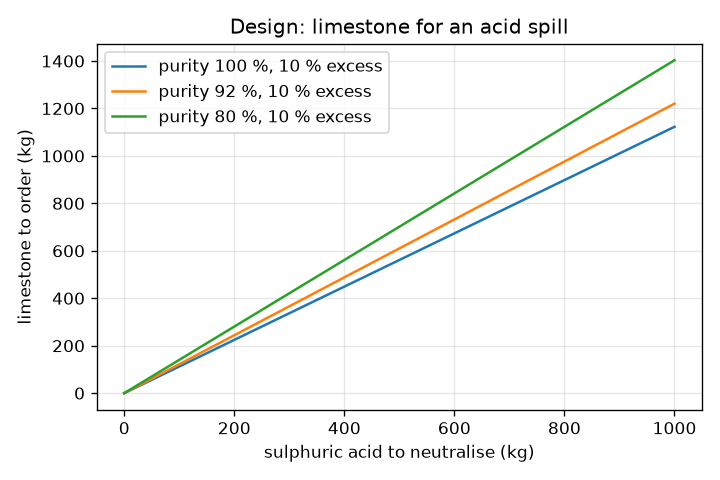
\includegraphics[width=0.85\linewidth]{figures/s02_limestone_design.png}\\\small Limestone to order against acid to neutralise, for three purities with 10 percent excess.\end{center}

\subsection*{E. Worked example}
How many grams of CO2 are produced when 16 g of CH4 burns completely in CH4 + 2 O2 -\textgreater{} CO2 + 2 H2O? Check that mass is conserved.
\begin{enumerate}[nosep]
\item M(CH4) = 12.011 + 4 * 1.008 = 16.043 g/mol, so n(CH4) = 16 / 16.043 = 0.9973 mol.
\item The coefficients of CH4 and CO2 are both 1, so n(CO2) = 0.9973 mol.
\item M(CO2) = 12.011 + 2 * 15.999 = 44.009 g/mol, so m(CO2) = 0.9973 * 44.009 = 43.89 g.
\item Mass check: O2 used = 2 * 0.9973 * 31.998 = 63.82 g and H2O formed = 2 * 0.9973 * 18.015 = 35.93 g. In: 16 + 63.82 = 79.82 g. Out: 43.89 + 35.93 = 79.82 g.
\end{enumerate}
\textbf{Answer.} 16 g of CH4 gives 43.9 g of CO2 (43.89 g with these atomic masses; rounding M(CH4) to 16.0 gives about 44.0 g). Mass in equals mass out: 79.82 g.

\subsection*{F. Questions}
\begin{enumerate}[nosep]
\item \textbf{Conceptual.} In CH4 + 2 O2 -\textgreater{} CO2 + 2 H2O the coefficients are 1 : 2 : 1 : 2. Does 1 g of CH4 need 2 g of O2? Explain.
\item \textbf{Numerical.} How many grams of NaCl do you need for 0.5 L of a 0.10 mol/L solution? How many NaCl formula units is that?
\item \textbf{Graph and simulation interpretation.} In the yield graph (16 g CH4), what is the slope of the rising part and where does the kink occur? Why is the graph flat afterwards?
\item \textbf{Design and optimisation challenge.} Design: 250 kg of sulphuric acid must be neutralised with limestone that is 90 percent CaCO3, with a 15 percent safety excess, in 25 kg bags. How many bags? How much CO2 is released at least? State the balanced equation.
\end{enumerate}

\section{Session 3: An automatic balancer and a reactor sweep}

\subsection*{A. Real-world problem}
A fertiliser plant turns nitrogen and hydrogen into ammonia. Before buying gas the engineer needs the exact ratio and the answer to one question: how much hydrogen does a tonne of ammonia need? Balancing by trial works for water, but a real reaction can have ten species, and some equations cannot be balanced at all or can be balanced in several ways. Atom conservation is a set of linear equations, so a computer can balance anything. This session is general education about an idealised model, not a plant design.

\subsection*{B. Concept and theory}
Take every species as a column and every element as a row. The entry is the number of atoms of that element in the species, with a plus sign for reactants and a minus sign for products. For ionic equations add one more row with the charge of each species (also signed). With coefficients c in a column vector, atom and charge conservation say A c = 0. The set of all such c is the null space of A; its dimension (the nullity) tells how many independent ways there are to balance. Nullity 1 gives a unique recipe up to a common factor; nullity 0 means the species cannot be balanced; nullity 2 or more means several independent recipes (not a unique answer). We find the null space with the singular value decomposition: right singular vectors whose singular value is zero span it. A unit-length vector is not a recipe, so we divide by the smallest non-zero entry, rationalise each entry with Fraction.limit\_denominator, multiply by the common denominator, divide by the greatest common divisor and make the signs positive, then verify A c = 0 exactly with integers. A physical reaction needs every coefficient to be positive. For a reactor, the feed ratio decides which reagent limits: with 1 mol of N2 and r mol of H2 the extent is min(1, r/3), and mass is conserved however the reagents are mixed.

\begin{itemize}[nosep]
\item A: element-by-species matrix (reactants +, products -) (atoms (counts))
\item c: vector of coefficients (no unit)
\item k: nullity: dimension of the null space of A (no unit)
\item r: feed ratio n(H2) / n(N2) (mol/mol)
\item xi: extent of reaction (mol)
\item conversion: fraction of the possible extent achieved (no unit (0 to 1))
\item S: sensitivity: percent change of the answer for 1 percent change of an atomic mass (percent per percent)
\end{itemize}

\begin{equation*}
A_{e,j}=\pm\,(\text{atoms of element }e\text{ in species }j)\qquad A_{q,j}=\pm\,(\text{charge of species }j)
\end{equation*}

\begin{equation*}
A\,\mathbf c=\mathbf 0\qquad \text{nullity }k=n_{\text{species}}-\operatorname{rank}A
\end{equation*}

\begin{equation*}
A=U\Sigma V^{\mathsf T}\;\Rightarrow\;\text{null space}=\operatorname{span}\{\mathbf v_j:\sigma_j\approx 0\}
\end{equation*}

\begin{equation*}
\xi=\min\!\left(n_{\mathrm{N_2}},\tfrac{1}{3}n_{\mathrm{H_2}}\right)\qquad n_{\mathrm{NH_3}}=2\xi
\end{equation*}

\begin{equation*}
m_{\mathrm{H_2}}=\frac{3\,M_{\mathrm{H_2}}}{2\,M_{\mathrm{NH_3}}}\,m_{\mathrm{NH_3}}
\end{equation*}

\begin{center}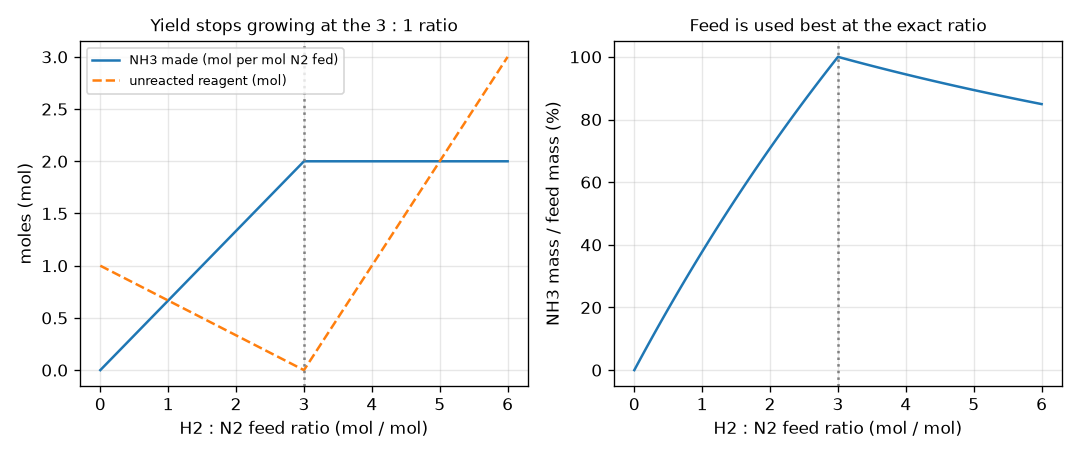
\includegraphics[width=0.85\linewidth]{figures/s03_feed_ratio_sweep.png}\\\small Ammonia made and reagent wasted against the H2 to N2 feed ratio, and the ammonia mass over feed mass.\end{center}

\subsection*{E. Worked example}
Balance Fe2O3 + Al -\textgreater{} Al2O3 + Fe with the null-space method and verify the result.
\begin{enumerate}[nosep]
\item Species columns in order: Fe2O3, Al, Al2O3, Fe. Rows in alphabetical order: Al, Fe, O. Reactants plus, products minus: A = [[0, 1, -2, 0], [2, 0, 0, -1], [3, 0, -3, 0]].
\item Row Al: b - 2c = 0. Row Fe: 2a - d = 0. Row O: 3a - 3c = 0. So c = a, b = 2a, d = 2a, one free number a, hence nullity 1 (3 independent rows, 4 columns).
\item Take a = 1: the null vector is (1, 2, 1, 2). The numpy SVD returns a unit-length multiple of it, (0.31, 0.63, 0.31, 0.63), which rationalises to the same integers.
\item Check by integers: A c = (0 + 2 - 2, 2 + 0 - 0 - 2, 3 + 0 - 3 - 0) = (0, 0, 0). Check by mass: 159.687 + 2 * 26.982 = 213.651 g and 101.961 + 2 * 55.845 = 213.651 g.
\end{enumerate}
\textbf{Answer.} Fe2O3 + 2 Al -\textgreater{} Al2O3 + 2 Fe; the nullity is 1 and A c = 0 exactly; total mass 213.651 g per mole of reaction on each side.

\subsection*{F. Questions}
\begin{enumerate}[nosep]
\item \textbf{Conceptual.} Why does a unique balanced equation correspond to a null space of dimension exactly 1? What would nullity 0 and nullity 2 mean?
\item \textbf{Numerical.} How many kilograms of hydrogen are needed for 250 kg of ammonia, assuming complete reaction? Check with a mass balance.
\item \textbf{Graph and simulation interpretation.} In the feed-ratio graph (left), why does the NH3 line become flat at ratio 3 while the red waste curve has a V shape with its minimum at 3?
\item \textbf{Design and optimisation challenge.} Design: a plant feeds 100 kmol/h of N2, but the hydrogen meter is only good to plus or minus 5 percent. Choose the hydrogen set-point ratio so that yield never falls below 99.5 percent of the possible ammonia, and report the worst-case hydrogen waste.
\end{enumerate}

\section{Real-world mini-project}
\textbf{Scale up the fertiliser recipe: hydrogen for one tonne of ammonia.} Ammonia for fertiliser is made by N2 + 3 H2 -\textgreater{} 2 NH3. A plant wants to make 1 tonne (1000 kg) of NH3. Use the Session 3 balancer to get the coefficients, then compute the hydrogen and nitrogen needed, check that the mass balance closes, and repeat the hydrogen estimate if only 90 percent of the possible reaction is achieved. Finally report how much the answer moves if the atomic mass of hydrogen in your table is 1 percent too high.

\section{The path ahead}
\begin{enumerate}[nosep]
\item \textbf{Session 4: Equations with many solutions.} A balancer that, for nullity 2 or more, returns the extreme positive integer solutions instead of just a basis.
\item \textbf{Session 5: Titration: from volumes to a concentration.} A calculator that turns titration volumes into a concentration with an uncertainty.
\item \textbf{Session 6: Recycle and purge.} A steady-state mass balance of a reactor, separator and recycle stream.
\item \textbf{Session 7: Equilibrium instead of complete reactions.} A solver for the equilibrium extent of a reaction with a given constant.
\item \textbf{Session 8: Animate the balancer.} An animation of any balanced reaction with mole and mass bars.
\end{enumerate}

\section{Answers and hints}

\subsection*{Session 1}
\begin{enumerate}[nosep]
\item \textbf{Conceptual.} Hint: What substance is H2O2? Which numbers may be changed when balancing? Solution: H2O2 is hydrogen peroxide, a different substance from water, so the equation no longer describes the same reaction. Small numbers inside a formula identify the substance and must never be changed; only the coefficients in front may be changed. The correct fix is the coefficient 2 in front of H2O (and a 2 in front of H2).
\item \textbf{Numerical.} Hint: Balance carbon first (1 and 1), then hydrogen, then oxygen last. Solution: CH4 + 2 O2 -\textgreater{} CO2 + 2 H2O. Left: 1 C, 4 H, 4 O. Right: 1 C, 4 H (2 H2O), and 2 + 2 = 4 O (one CO2 and two H2O). The counts agree for every element. Units: all counts are numbers of atoms.
\item \textbf{Graph and simulation interpretation.} Hint: Find where the H line (2c) reaches 4 and where the O line (c) reaches 2. Solution: They meet at c = 2: H right is 2c = 4 = H left and O right is c = 2 = O left. At c = 1 the right side has only 2 H and 1 O, too few; at c = 3 it has 6 H and 3 O, too many. Both elements are balanced at the same single value, which is why a solution exists.
\item \textbf{Design and optimisation challenge.} Hint: The recipe 2 : 1 : 2 is repeated 6 times for 12 waters. For the second part, see which ingredient runs out first. Solution: 12 waters is 6 times the recipe, so 12 H2 and 6 O2. With 7 O2 you can make at most 14 water molecules, which needs 14 H2. Hydrogen (20) is enough, so oxygen runs out first: 14 H2O are made and 6 H2 are left over. Assumption: the reaction goes to completion. The ingredient that runs out first is called the limiting reagent (Session 2).
\end{enumerate}

\subsection*{Session 2}
\begin{enumerate}[nosep]
\item \textbf{Conceptual.} Hint: Are the coefficients mole ratios or mass ratios? Compare M(CH4) and M(O2). Solution: No. The coefficients are ratios of moles (molecules), not of grams. One mole of CH4 (16.043 g) needs two moles of O2 (63.996 g), so 1 g of CH4 needs about 3.99 g of O2. Convert to moles first, apply the ratio, then convert back to grams.
\item \textbf{Numerical.} Hint: n = c * V, then m = n * M. M(NaCl) = 22.990 + 35.45. Solution: n = 0.10 * 0.5 = 0.050 mol. M(NaCl) = 58.44 g/mol, so m = 0.050 * 58.44 = 2.922 g (about 2.9 g). Formula units = 0.050 * 6.022e23 = 3.0e22. Check: 2.922 / 58.44 = 0.050 mol.
\item \textbf{Graph and simulation interpretation.} Hint: The slope is the CO2 mass per gram of O2 before methane is used up: M(CO2) / (2 M(O2)). Solution: Slope = 44.009 / (2 * 31.998) = 0.688 g of CO2 per g of O2. The kink is at 63.8 g of O2 (2 mol per mol CH4 times 0.9973 mol * 31.998 g/mol). Beyond it methane is the limiting reagent, so extra oxygen cannot make more CO2: the plateau is 43.89 g.
\item \textbf{Design and optimisation challenge.} Hint: CaCO3 + H2SO4 -\textgreater{} CaSO4 + H2O + CO2 is 1 : 1. Pure CaCO3 mass = acid mass * M(CaCO3) / M(H2SO4); then apply the excess and divide by the purity. Solution: M(H2SO4) = 98.072 g/mol and M(CaCO3) = 100.086 g/mol. Pure CaCO3 = 250 * 100.086 / 98.072 = 255.1 kg. With 15 percent excess: 293.4 kg of CaCO3; at 90 percent purity this is 326.0 kg of limestone. 326.0 / 25 = 13.04, so 14 bags (350 kg). CO2 from the acid actually neutralised: 250 / 98.072 * 44.009 = 112.2 kg (roughly 60 cubic metres of gas, so work outdoors and keep the area ventilated). Assumptions: complete reaction, inert impurities; the excess limestone does not react further. Trade-off: more excess is safer for the spill but costs more and leaves more solid to dispose of.
\end{enumerate}

\subsection*{Session 3}
\begin{enumerate}[nosep]
\item \textbf{Conceptual.} Hint: Count free numbers: how many coefficients can you choose before the rest are fixed? Solution: Nullity is the number of free numbers left after all conservation equations are used. With nullity 1 you choose one number (the overall scale) and everything else follows, so the recipe is unique up to scaling by a common factor. Nullity 0 means only c = 0 satisfies the equations: the species cannot conserve every element (for example H2 + O2 -\textgreater{} NaCl). Nullity 2 means two independent recipes exist and any positive combination also balances, so the equation is not uniquely balanced (for example H2 + O2 -\textgreater{} H2O + H2O2).
\item \textbf{Numerical.} Hint: m(H2) = 1.5 * M(H2) / M(NH3) * m(NH3) with M(H2) = 2.016 and M(NH3) = 17.031 g/mol. Solution: m(H2) = 1.5 * 2.016 / 17.031 * 250 = 44.39 kg. Nitrogen: 28.014 / (2 * 17.031) * 250 = 205.6 kg. Check: 44.39 + 205.6 = 250.0 kg. Units: kg, since the molar-mass ratio has no unit.
\item \textbf{Graph and simulation interpretation.} Hint: Which reagent limits on each side of 3? Solution: Below 3, hydrogen limits: every extra mole of H2 makes 2/3 mol more NH3 (the rising line) and the leftover is nitrogen, which shrinks. Above 3, nitrogen limits: the NH3 is fixed at 2 mol and every extra H2 is waste, so the waste grows. At exactly 3 nothing is left over, so waste is 0, the minimum of the V.
\item \textbf{Design and optimisation challenge.} Hint: The lowest actual ratio is set-point * 0.95; yield is min(1, r / 3). Then the highest ratio is set-point * 1.05. Solution: We need 0.95 * set-point / 3 \textgreater{}= 0.995, so set-point \textgreater{}= 3.142; take 3.15. Lowest ratio = 2.9925, yield 99.75 percent of the possible. Highest ratio = 3.3075, so 0.3075 mol of H2 per mol N2 is wasted, about 9.3 percent of the fed hydrogen. Trade-off: tighter metering lets the set-point move towards 3 and waste less hydrogen; a lower set-point wastes less but risks lost yield. Assumption: complete conversion and no recycle (a real plant recycles unreacted gas).
\end{enumerate}

\section{How to join}
Read \texttt{CONTRIBUTING.md} in the repository, then pick an issue labelled \texttt{good first issue}. Repository: \url{https://github.com/KrunalPanchal1995/openmole}

\end{document}
